\documentclass[11pt]{article}

\usepackage[margin=1in]{geometry}
\usepackage{amsmath,amssymb,amsthm}
\usepackage{mathpazo}
\usepackage{microtype}
\usepackage{booktabs}
\usepackage{tabularx}
\usepackage[dvipsnames]{xcolor}
\usepackage{enumitem}
\usepackage{fancyhdr}
\usepackage[most]{tcolorbox}
\usepackage{pgfplots}
\usepackage[round,authoryear]{natbib}
\usepackage[colorlinks=true,linkcolor=NavyBlue,citecolor=NavyBlue,urlcolor=NavyBlue]{hyperref}
\usepgfplotslibrary{groupplots}
\pgfplotsset{compat=1.16}

\definecolor{navy}{HTML}{1F3A5F}
\definecolor{cEq}{HTML}{1F3A5F}
\definecolor{cOp}{HTML}{C8553D}
\definecolor{cMk}{HTML}{8A8A8A}
\definecolor{cBl}{HTML}{2E8B57}
\newtheorem{proposition}{Proposition}
\theoremstyle{definition}
\newtheorem{definition}{Definition}

\newcommand{\E}{\mathbb{E}}
\newcommand{\Var}{\operatorname{Var}}
\newcommand{\Cov}{\operatorname{Cov}}
\newcommand{\sgn}{\operatorname{sgn}}
\newcommand{\1}{\mathbf{1}}
\newcommand{\F}{\mathcal{F}}

\pagestyle{fancy}
\fancyhf{}
\lhead{\small\textsc{Post-Earnings Drift: Mechanism, Evidence, and a Two-Book Strategy}}
\rhead{\small\thepage}
\renewcommand{\headrulewidth}{0.4pt}
\setlist{itemsep=2pt,topsep=4pt}

\pgfplotsset{
  pead/.style={width=\linewidth,height=6.2cm,tick label style={font=\footnotesize},
    label style={font=\small},legend style={font=\footnotesize,draw=none,fill=none},
    grid=major,grid style={gray!25},every axis plot/.append style={line width=0.9pt}}
}

\title{\vspace{-1.2cm}\textbf{Post-Earnings-Announcement Drift:\\[2pt]
Mechanism, Evidence, and a Hedged Equity--Options Strategy}}
\author{Hrudith L.\\[2pt] \small PEAD Trading Research}
\date{\today}

\begin{document}
\maketitle
\thispagestyle{empty}

\begin{abstract}
\noindent
Markets underreact to earnings news. A firm's price keeps moving in the direction of its
earnings surprise for weeks after the announcement. We formalize this as gradual
incorporation of information by heterogeneously attentive investors, and we show it is
the source of profit for two complementary strategies. The evidence is a 182{,}712-event
sample (1996--2013) in which the top-minus-bottom surprise-decile spread is $+3.05\%$
over 60 trading days ($t=5.25$, clustered by quarter) and $+3.76\%$ ($t=9.25$) after
controlling for size and book-to-market. The same ordering appears in option premia,
amplified by the options' elasticity ($\approx4.7\times$). The first strategy is a
market-, sector- and size-neutral equity long/short book that earns the drift linearly:
$12.2\%$ a year at $12.2\%$ volatility, with no market beta. The second is a long-only
options book that earns the same drift convexly. It picks, for each event, the contract that
maximizes expected log growth, and it sizes the book as a deeply fractional Kelly portfolio:
$12.3\%$ a year at $3.3\%$ volatility. The two books have a daily return correlation of
$-0.05$. Together they deliver an equal-weight Sharpe ratio of $1.9$ and a maximum drawdown of
$-18.5\%$. We derive the properties that make each book work: the neutrality of the equity
weights, the capacity trade-off, the equivalence of Kelly ranking to Sharpe ranking, and the
role of breadth in the options book's Sharpe ratio.
\end{abstract}

\begin{tcolorbox}[colback=navy!4,colframe=navy,title=\textbf{Summary of results (backtest, 1996--2013, \$10M initial capital, net of modeled costs)},fonttitle=\small,left=4pt,right=4pt,top=3pt,bottom=3pt]
\small
\begin{tabularx}{\linewidth}{@{}Xrrrrr@{}}
\toprule
Book & Ann.\ return & Ann.\ vol & Sharpe & Max DD & Mkt.\ beta \\
\midrule
Equity long/short (market-hedged) & 12.15\% & 12.20\% & 1.00 & $-36.5\%$ & $-0.015$ \\
Options (growth-optimal) & 12.26\% & 3.33\% & 3.49 & $-17.4\%$ & $0.034$ \\
50/50 combination, 1998--2013$^\dagger$ & 12.73\% & 6.48\% & 1.88 & $-18.5\%$ & -- \\
\bottomrule
\end{tabularx}
\vspace{2pt}
{\footnotesize $^\dagger$Computed from the two books' daily return series, rebalanced daily.
All figures are hypothetical backtest results.}
\end{tcolorbox}

\tableofcontents
\newpage

%=====================================================================================
\section{Introduction}
%=====================================================================================

When a firm reports earnings that differ from expectations, its price does not adjust
fully on the announcement. Over the following weeks it keeps moving in the direction of the
surprise \citep{BallBrown1968,BernardThomas1989,BernardThomas1990}. This post-earnings-announcement
drift (PEAD) is attributed to underreaction and investor inattention
\citep{HongStein1999,HirshleiferLimTeoh2009,DellaVignaPollet2009}, and it survives because
the capital that could remove it is costly to deploy \citep{ShleiferVishny1997,Mendenhall2004}.

This paper has one thesis: PEAD is a gradual transfer of value from slow to fast
investors, and it can be harvested in two structurally different ways. The paper is organized
around three questions.
\begin{enumerate}[label=(\roman*)]
  \item \textbf{Where does the money come from?} Section~\ref{sec:mechanism} gives a model
        of gradual incorporation. It predicts the shape of the drift in time, its dependence
        on frictions, and its amplification in options.
  \item \textbf{Does the phenomenon exist?} Section~\ref{sec:evidence} tests every prediction
        of the model before any strategy is built: clustering-robust significance, size and
        value controls, cross-sectional heterogeneity, and confirmation in a second market.
  \item \textbf{How well does it trade?} Sections~\ref{sec:equity}--\ref{sec:combined} build
        a linear equity book and a convex options book, show how each converts the drift
        into return, and evaluate them separately and together.
\end{enumerate}

%=====================================================================================
\section{Where the money comes from}\label{sec:mechanism}
%=====================================================================================

\subsection{Gradual incorporation of a surprise}

Let firm $i$ announce earnings at day $0$ with standardized surprise $z_i$, normalized to
have mean zero and unit variance within its announcement quarter. Suppose the surprise
changes the firm's full-information value by $\lambda z_i$ (in return units, with $\lambda>0$
the information content of a unit surprise). The price embeds only a fraction $\phi(d)$ of
that revision $d$ days after the announcement, with $0\le\phi(0)<1$ and $\phi(d)\uparrow1$.
Then the market-adjusted cumulative return to horizon $h$, measured from the day after the
announcement, is
\begin{equation}
  \E\big[\mathrm{CAR}_i(h)\mid z_i\big]=\lambda\,\big[\phi(h)-\phi(0)\big]\,z_i,
  \label{eq:drift}
\end{equation}
so the cross-sectional \emph{spread} between the top and bottom surprise groups is
\begin{equation}
  \Delta(h)=\E[\mathrm{CAR}\mid \text{top}]-\E[\mathrm{CAR}\mid\text{bottom}]
  =\lambda\,\big[\phi(h)-\phi(0)\big]\,(\bar z_{\text{top}}-\bar z_{\text{bottom}}).
  \label{eq:spread}
\end{equation}
The spread is the economic object that both strategies harvest. It is non-negative,
increasing, and bounded by $\lambda(1-\phi(0))(\bar z_{\text{top}}-\bar z_{\text{bottom}})$.

\paragraph{Microfoundation: heterogeneous attention.}
Suppose a fraction of capital updates at an idiosyncratic Poisson rate $\kappa$, with
$\kappa$ distributed across investors according to a distribution $G$. Then
$\phi(d)=\phi(0)+(1-\phi(0))\int(1-e^{-\kappa d})\,dG(\kappa)$. If $G$ is Gamma with shape $k$
and rate $\theta$,
\begin{equation}
  \phi(d)=\phi(0)+\big(1-\phi(0)\big)\Big[1-\big(1+d/\theta\big)^{-k}\Big].
  \label{eq:phi}
\end{equation}
A mixture of speeds makes incorporation \emph{concave but slow}: fast updaters finish within
days, while inattentive investors take months. A single speed would produce an exponential
approach and a spread that flattens within a few multiples of $1/\kappa$. Equation
\eqref{eq:phi} instead produces a spread that keeps rising at a decreasing rate, which is the
shape observed in Section~\ref{sec:evidence}.

\subsection{Limits to arbitrage determine where the drift is largest}

Informed capital closes the gap only until the marginal profit no longer covers the
marginal cost of carrying the trade. Let $\xi_i$ be the per-day all-in cost of holding a
position in firm $i$ (spread, impact, borrow, and the idiosyncratic risk the arbitrageur must
bear), and let $\alpha_i(d)=\lambda\phi'(d)|z_i|$ be the daily drift. Arbitrage capital
flows in while $\alpha_i(d)>\xi_i$ and stops when $\alpha_i(d)\approx\xi_i$. The drift that
survives is therefore increasing in $\xi_i$: it is largest in small, illiquid, hard-to-short
stocks. This is a sharp, testable cross-sectional prediction, which
Section~\ref{sec:evidence} confirms: the spread is monotone decreasing in firm size.

\subsection{Why options carry a larger signal}

An option is a leveraged claim on the underlying. For a call with price $C$ and delta $\Delta_c$
on a stock priced at $S$, a small stock return $r$ changes the option's return on premium by
approximately $\Omega\, r$, where
\begin{equation}
  \Omega=\frac{\Delta_c\,S}{C}
  \label{eq:omega}
\end{equation}
is the option's elasticity. At the money, $C\approx0.4\,S\sigma\sqrt{T}$, so
$\Omega\approx\Delta_c/(0.4\,\sigma\sqrt T)$. With $\Delta_c\approx0.5$, maturity near four
months and annual volatility $\sigma\in[0.35,0.45]$, this gives $\Omega\approx 4.8$--$6.2$.
The drift in the option's premium is therefore $\Omega$ times the drift in the stock, less a
decay and volatility cost that grows with the holding period. Two further features matter.
Losses on a purchased option are capped at the premium, and the payoff is convex in the
stock price, so a few large moves contribute disproportionately to growth.

\subsection{Two ways to earn the same spread}

The model suggests two harvesting designs.
\begin{itemize}
  \item \textbf{Linear.} Take long positions in positive surprises and short positions in
        negative surprises, and hedge everything that is not the drift. Expected profit is
        $\sum_i w_i\,\E[\mathrm{CAR}_i]$ for weights $w_i$. This is a breadth strategy:
        profit is roughly proportional to the number of independent bets, and risk comes
        from residual common factors.
  \item \textbf{Convex.} Buy the option that gives the most favorable growth per unit of
        capital at risk. Each event is a bounded-loss bet. Profit again scales with breadth,
        but the payoff skew is positive and the maximum loss is known in advance.
\end{itemize}
The two books earn from the same event but through different return distributions. The
equity book is exposed to its short leg in a junk rally, and the options book is not. This
is why they diversify each other (Section~\ref{sec:combined}).

%=====================================================================================
\section{Evidence that the drift exists}\label{sec:evidence}
%=====================================================================================

\subsection{Data and the surprise measure}

The sample combines I/B/E/S analyst consensus and actuals, CRSP daily returns and the
value-weighted market return $r_{m,t}$, Compustat book equity, and OptionMetrics daily option
quotes. An event is a firm-quarter earnings announcement from 1996 to 2013. The surprise is
\begin{equation}
  \mathrm{SUE}_i=\frac{A_i-F_i}{s_i},
\end{equation}
with $A_i$ realized earnings per share, $F_i$ the most recent consensus forecast made before the
announcement, and $s_i>0$ a firm-specific scale. The headline sample has 182{,}712 events on
6{,}766 firms across $Q=72$ announcement quarters. For event $i$ announced at day $0$, the
market-adjusted return to horizon $h$ is
\[
  \mathrm{CAR}_i(h)=\prod_{k=1}^{h}(1+r_{i,k})-\prod_{k=1}^{h}(1+r_{m,k}),
\]
accrued from the day \emph{after} the announcement, so the announcement-day reaction is
excluded from the drift. Within each quarter, events are ranked by SUE into percentile
$u_i\in(0,1]$ and assigned to deciles $D_i=\min(\lceil10u_i\rceil,10)$.

\subsection{Inference under earnings-season clustering}

Firms announcing in the same season share common shocks, so event-level standard errors
overstate precision. We use the Fama--MacBeth estimator \citep{FamaMacBeth1973} with the
announcement quarter as the unit of observation. For an event-level quantity $x_i$ and event
set $\mathcal S$, with $\mathcal I_q$ the events in quarter $q$,
\begin{equation}
  \bar x_q=\frac{1}{|\mathcal S\cap\mathcal I_q|}\sum_{i\in\mathcal S\cap\mathcal I_q}x_i,\qquad
  \hat\mu=\frac1Q\sum_{q=1}^{Q}\bar x_q,\qquad
  \widehat{\mathrm{SE}}(\hat\mu)=\frac{1}{\sqrt Q}\Big[\tfrac{1}{Q-1}\textstyle\sum_q(\bar x_q-\hat\mu)^2\Big]^{1/2}.
  \label{eq:fm}
\end{equation}
The estimator is consistent under arbitrary dependence within a quarter. The spread is formed
quarter by quarter, $\Delta_q(h)=\overline{\mathrm{CAR}}_{q,D10}(h)-\overline{\mathrm{CAR}}_{q,D1}(h)$,
so its standard error reflects the fact that both legs are drawn from the same cross-section.

\subsection{The drift in equities}

\begin{figure}[t]\centering
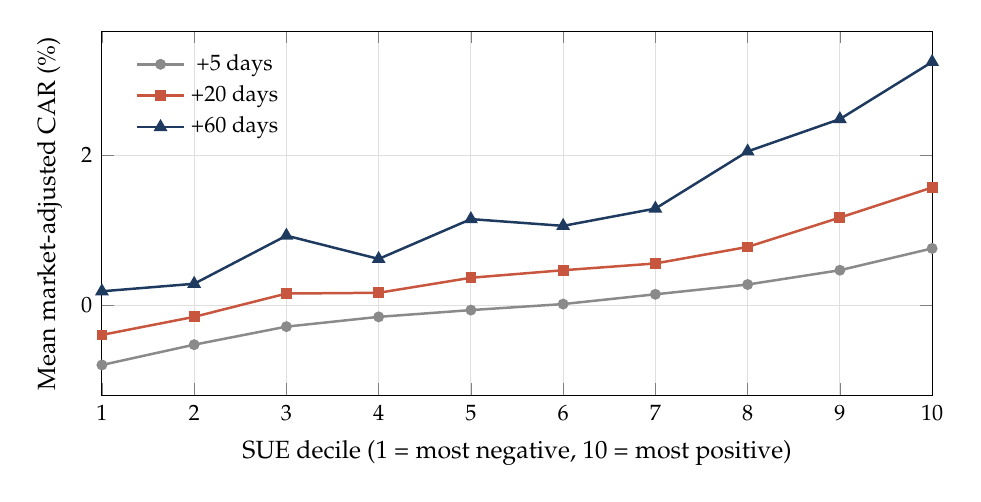
\begin{tikzpicture}
\begin{axis}[pead,xlabel={SUE decile (1 = most negative, 10 = most positive)},
  ylabel={Mean market-adjusted CAR (\%)},xmin=1,xmax=10,xtick={1,...,10},
  legend pos=north west]
\addplot[color=cMk,mark=*,mark size=1.5pt] coordinates {(1,-0.79)(2,-0.52)(3,-0.28)(4,-0.15)(5,-0.06)(6,0.02)(7,0.15)(8,0.28)(9,0.47)(10,0.76)};
\addplot[color=cOp,mark=square*,mark size=1.5pt] coordinates {(1,-0.39)(2,-0.15)(3,0.16)(4,0.17)(5,0.37)(6,0.47)(7,0.56)(8,0.78)(9,1.17)(10,1.57)};
\addplot[color=cEq,mark=triangle*,mark size=2pt] coordinates {(1,0.19)(2,0.29)(3,0.93)(4,0.62)(5,1.15)(6,1.06)(7,1.29)(8,2.05)(9,2.48)(10,3.24)};
\legend{+5 days,+20 days,+60 days}
\end{axis}
\end{tikzpicture}
\caption{Mean market-adjusted cumulative return by SUE decile at three horizons. The profile
tilts upward with surprise, and the tilt steepens as the horizon lengthens, as
equation~\eqref{eq:drift} predicts.}\label{fig:decile}
\end{figure}

\begin{table}[t]\centering\small
\caption{Mean market-adjusted CAR (\%) by SUE decile and horizon (Fama--MacBeth means over 72 quarters).}\label{tab:deciles}
\begin{tabular}{lrrrrrr}
\toprule
Decile & $+1$d & $+5$d & $+10$d & $+20$d & $+40$d & $+60$d \\
\midrule
D1 (most negative) & $-0.47$ & $-0.79$ & $-0.65$ & $-0.39$ & $-0.06$ & $+0.19$ \\
D2 & $-0.32$ & $-0.52$ & $-0.42$ & $-0.15$ & $+0.11$ & $+0.29$ \\
D3 & $-0.22$ & $-0.28$ & $-0.18$ & $+0.16$ & $+0.42$ & $+0.93$ \\
D4 & $-0.11$ & $-0.15$ & $-0.08$ & $+0.17$ & $+0.34$ & $+0.62$ \\
D5 & $+0.03$ & $-0.06$ & $+0.01$ & $+0.37$ & $+0.66$ & $+1.15$ \\
D6 & $+0.02$ & $+0.02$ & $+0.15$ & $+0.47$ & $+0.70$ & $+1.06$ \\
D7 & $+0.13$ & $+0.15$ & $+0.32$ & $+0.56$ & $+0.81$ & $+1.29$ \\
D8 & $+0.14$ & $+0.28$ & $+0.37$ & $+0.78$ & $+1.27$ & $+2.05$ \\
D9 & $+0.26$ & $+0.47$ & $+0.78$ & $+1.17$ & $+1.62$ & $+2.48$ \\
D10 (most positive) & $+0.36$ & $+0.76$ & $+1.05$ & $+1.57$ & $+2.30$ & $+3.24$ \\
\bottomrule
\end{tabular}
\end{table}

Table~\ref{tab:deciles} and Figure~\ref{fig:decile} show the canonical pattern. Decile means
are ordered by surprise, and the top-minus-bottom spread widens with the horizon, from $0.83\%$
at one day to $3.05\%$ at 60 days (Table~\ref{tab:spreads}). Every clustered $t$-statistic
exceeds $5.2$. A one-time reaction that merely differed across deciles would produce a flat
spread. A rising spread is the signature of gradual incorporation.

\paragraph{The shape of the drift.}
Over the six horizons, the characteristic-adjusted spread follows
$\Delta(h)\approx0.77\,h^{0.37}$ percent ($R^2=0.97$), and the market-adjusted spread follows
$0.86\,h^{0.29}$ ($R^2=0.96$). A single-speed exponential approach fits visibly worse
($R^2\approx0.72$--$0.80$). Growth that is a power of the horizon and has not saturated by day 60
is consistent with the heterogeneous-attention mixture \eqref{eq:phi}, in which the
unincorporated fraction decays as a power and there is no single time scale.

\subsection{Is the drift a risk premium in disguise?}

Extreme-bad-news firms tend to be small, high book-to-market firms that earn a size and value
premium. In market-adjusted terms the worst decile recovers toward zero and turns positive by day 60, which raises the
possibility that part of the drift is compensation for risk rather than mispricing. We test
this with a characteristic benchmark in the spirit of \citet{DGTW1997}. Each event is assigned to
a cell $c(i)$ defined by quarter, size quintile, and book-to-market tercile, and its return
is measured against the average of its cell-mates, excluding itself:
\begin{equation}
  \widetilde{\mathrm{CAR}}_i(h)=\mathrm{CAR}_i(h)-\frac{\sum_{j\in c(i)}\mathrm{CAR}_j(h)-\mathrm{CAR}_i(h)}{n_{c(i)}-1}.
  \label{eq:loo}
\end{equation}
Leaving the event out of its own benchmark prevents its return from shrinking toward zero in
thin cells. If the drift were a risk premium, the adjustment would shrink the spread. It does
the opposite: the 60-day spread rises from $3.05\%$ to $3.76\%$ ($t=9.25$), and the worst decile
no longer recovers (its adjusted 60-day return is $-1.71\%$). The apparent reversal of the worst decile was a size/value premium
sitting on top of the drift. Removing it reveals the drift in full (Table~\ref{tab:spreads},
Figure~\ref{fig:spreads}).

\begin{table}[t]\centering\small
\caption{Top-minus-bottom decile spread by horizon, with quarter-clustered $t$-statistics.
Equity columns use the full sample. Option columns use the option-matched subsample and
measure the percentage return on premium of a near-the-money contract held at its mid price.}\label{tab:spreads}
\begin{tabular}{l rr rr rr rr rr}
\toprule
 & \multicolumn{2}{c}{Mkt-adj.\ equity} & \multicolumn{2}{c}{Size/BM-adj.\ equity} & \multicolumn{2}{c}{Call} & \multicolumn{2}{c}{Put} & \multicolumn{2}{c}{Straddle}\\
\cmidrule(lr){2-3}\cmidrule(lr){4-5}\cmidrule(lr){6-7}\cmidrule(lr){8-9}\cmidrule(lr){10-11}
Horizon & $\hat\mu$ & $t$ & $\hat\mu$ & $t$ & $\hat\mu$ & $t$ & $\hat\mu$ & $t$ & $\hat\mu$ & $t$\\
\midrule
$+1$d  & 0.83 & 10.90 & 0.80 & 11.41 & 4.01 & 13.33 & $-2.49$ & $-13.21$ & 0.27 & 3.31\\
$+5$d  & 1.54 & 12.23 & 1.59 & 14.21 & 8.03 & 13.27 & $-5.11$ & $-13.04$ & 0.77 & 4.61\\
$+10$d & 1.70 & 10.17 & 1.79 & 12.30 & 9.54 & 11.87 & $-5.86$ & $-13.01$ & 1.24 & 4.87\\
$+20$d & 1.96 & 8.74  & 2.18 & 12.09 & 11.29 & 8.34 & $-6.46$ & $-7.91$ & 2.18 & 4.97\\
$+40$d & 2.36 & 5.64  & 2.79 & 9.68  & 11.76 & 5.67 & $-8.27$ & $-6.64$ & 2.80 & 5.10\\
$+60$d & 3.05 & 5.25  & 3.76 & 9.25  & 14.38 & 4.69 & $-10.79$ & $-6.29$ & 3.98 & 5.22\\
\bottomrule
\end{tabular}
\end{table}

\subsection{The cross-section of the drift}

If frictions sustain the drift, it should differ across stocks in a predictable way. We test
this by computing the 60-day quarterly spread series separately within each group and testing
equality of means with a one-way ANOVA.
\begin{itemize}
  \item \textbf{Industry (Fama--French 12).} $F=0.30$, $p=0.99$. The spread is statistically
        indistinguishable across industries, so one drift model applies to the whole cross-section.
  \item \textbf{Size.} $F=6.50$, $p<10^{-4}$. The spread falls monotonically from $6.71\%$
        ($t=5.43$) in the smallest size quintile to $1.60\%$ ($t=2.41$) in the largest. This is the
        prediction of Section~\ref{sec:mechanism}: the drift is greatest where arbitrage is most
        expensive. Size is therefore a first-order determinant of the signal's value, and a
        strategy must neutralize it, not simply load on it.
\end{itemize}

\subsection{Confirmation in a second market}

If PEAD is a real mispricing of the stock, it must appear in the price of a leveraged claim
on that stock. For each event with listed options we take, on the announcement day, the call
(put) with delta nearest $+0.5$ ($-0.5$) and at least 95 days to expiry. We hold it at its mid
price to each horizon. The call spread is $+14.38\%$ of premium at 60 days ($t=4.69$) and the
put spread is $-10.79\%$ ($t=-6.29$), the mirror image (Table~\ref{tab:spreads}).

\paragraph{Magnitude check.} The ratio of the 60-day call spread to the stock spread is
$14.38/3.05\approx4.7$. This is just below the elasticity band $\Omega\in[4.8,6.2]$ from
equation~\eqref{eq:omega}, as expected once the option's time decay acts over 60 days. The
options market carries the same directional signal scaled by leverage, so the stock and
option evidence agree quantitatively as well as in sign.

\paragraph{Direction versus volatility.} A long straddle has roughly zero delta and isolates
the non-directional component. Its 60-day spread is $+3.98\%$ ($t=5.22$), about a quarter of
the call spread. Extreme-surprise names carry some excess volatility, but the dominant effect
is directional.

\begin{figure}[t]\centering
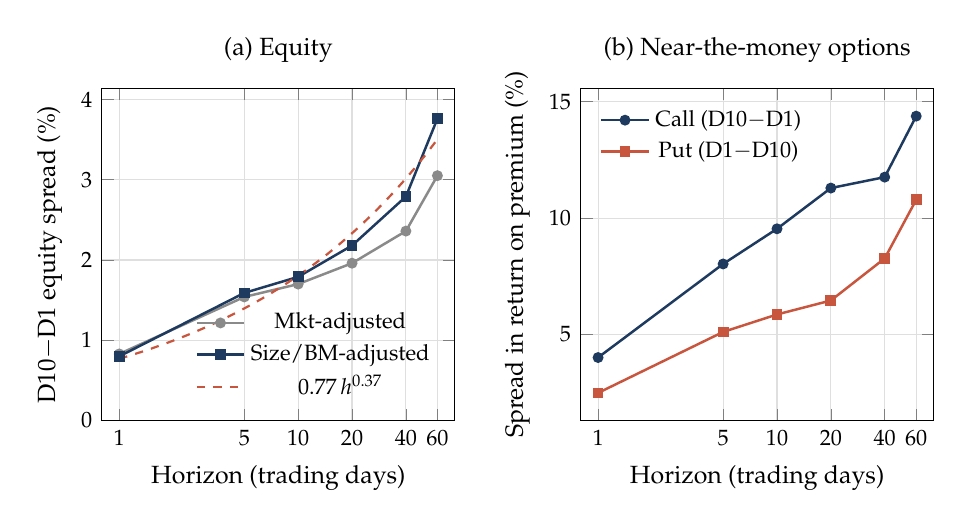
\begin{tikzpicture}
\begin{groupplot}[group style={group size=2 by 1,horizontal sep=1.6cm},
  pead,width=0.5\linewidth,height=5.8cm,xmode=log,xtick={1,5,10,20,40,60},
  xticklabels={1,5,10,20,40,60},xlabel={Horizon (trading days)},xmin=0.8,xmax=75]
\nextgroupplot[ylabel={D10$-$D1 equity spread (\%)},ymin=0,legend pos=south east,title={\small(a) Equity}]
\addplot[color=cMk,mark=*,mark size=1.5pt] coordinates {(1,0.83)(5,1.54)(10,1.70)(20,1.96)(40,2.36)(60,3.05)};
\addplot[color=cEq,mark=square*,mark size=1.5pt] coordinates {(1,0.80)(5,1.59)(10,1.79)(20,2.18)(40,2.79)(60,3.76)};
\addplot[color=cOp,dashed,domain=1:60,samples=30,line width=0.8pt] {0.77*x^0.37};
\legend{Mkt-adjusted,Size/BM-adjusted,$0.77\,h^{0.37}$}
\nextgroupplot[ylabel={Spread in return on premium (\%)},title={\small(b) Near-the-money options},legend pos=north west]
\addplot[color=cEq,mark=*,mark size=1.5pt] coordinates {(1,4.01)(5,8.03)(10,9.54)(20,11.29)(40,11.76)(60,14.38)};
\addplot[color=cOp,mark=square*,mark size=1.5pt] coordinates {(1,2.49)(5,5.11)(10,5.86)(20,6.46)(40,8.27)(60,10.79)};
\legend{Call (D10$-$D1),Put (D1$-$D10)}
\end{groupplot}
\end{tikzpicture}
\caption{Spread by horizon (log scale). (a) Equity, with the fitted power law. (b) Option
premia: the same rising profile, amplified.}\label{fig:spreads}
\end{figure}

\subsection{When to stop holding: the decay of the drift}

A trading rule must decide when the marginal day of holding stops paying. Let $a(H)$ be the
expected abnormal return from holding a position for $H$ days, net of the entry and exit
cost $k$. When capital is recycled into the next opportunity, the quantity to maximize is the
average net return per capital-day,
\begin{equation}
  \mathcal Y(H)=\frac{a(H)-k}{H},\qquad a(H)=\lambda|z|\big[\phi(H)-\phi(0)\big].
  \label{eq:holding}
\end{equation}
The first-order condition is $a'(H^\ast)=\mathcal Y(H^\ast)$: hold until the marginal daily drift
falls to the average daily net yield. Because $\phi$ is concave, $a'$ is decreasing, and
$H^\ast$ is unique whenever the total drift exceeds the cost (Appendix~\ref{app:proofs}).
Higher trading costs lengthen $H^\ast$, because a longer hold is needed to amortize them.
The empirical analogue used in the equity book estimates, for each group of events, the
first day on which the smoothed daily drift falls below a small fraction of its own peak.
Across groups, holding periods range from about six weeks to several months.

%=====================================================================================
\section{Strategy I: the market-neutral equity book}\label{sec:equity}
%=====================================================================================

\subsection{From signal to portfolio}

The book goes long positive surprises and short negative ones, with size increasing in the
strength of the surprise, and it holds each position for the decay time $H$ of
Section~\ref{sec:evidence}. Write $\delta_i=u_i-\tfrac12\in(-\tfrac12,\tfrac12]$ for a
centered within-quarter rank. The book trades only the two tails of the surprise
distribution, with conviction rising linearly in the distance from the center.

\begin{definition}[Rank-proportional, sector- and size-neutral weights]\label{def:weights}
For a trimming threshold $\tau$ and a tilt $\gamma$, define the conviction
$t_i=\1\{|\delta_i|>\tau\}\,\sgn(\delta_i)\,(2|\delta_i|)^{\gamma}$. For quarter $q$ and side
$\sigma\in\{+,-\}$, let $\mathcal{G}_{q\sigma}$ be the set of occupied groups, where a group
is a pair (industry, size bucket), and $N_{q\sigma}=|\mathcal G_{q\sigma}|$. The weights are
\begin{equation}
  \tilde w_i=\frac{t_i}{\sum_{j\in g(i)}|t_j|}\cdot\frac{1}{N_{q\sigma}},\qquad
  w_i=\frac{\tilde w_i}{2\,\overline{|\tilde w|}},
  \label{eq:weights}
\end{equation}
where $\overline{|\tilde w|}$ is a global normalizing constant.
\end{definition}

Within a group the weight is proportional to conviction, and each group receives the same
total weight on each side. The construction targets the two sources of unpriced risk that
the evidence identified: industry concentration and size, which is the dimension along
which the drift itself varies.

\begin{proposition}[Neutrality]\label{prop:neutral}
For every quarter's entry cohort:
(a) the long and short sides have equal gross weight, so the cohort is dollar-neutral;
(b) each occupied (industry, size) group receives exactly $1/N_{q\sigma}$ of its side's gross;
(c) net exposure to industry $k$ equals $\big(n^{+}_{k}/N_{q+}-n^{-}_{k}/N_{q-}\big)$ times
the global constant, where $n^\sigma_k$ is the number of occupied size buckets of industry $k$
on side $\sigma$. It vanishes whenever both sides occupy the same groups, and the same holds
for size.
\end{proposition}

\subsection{Where the P\&L comes from}

Position $i$ has dollar notional $n_i=w_i\,b\,V$, where $V$ is the book's capital and $b$ a
scale. Because returns are measured against the market, each stock position is economically
paired with an offsetting index position. The daily P\&L is
\begin{equation}
  \Pi_t=\sum_{i\ \text{open at }t}n_i\,(r_{i,t}-r_{m,t})\;-\;\sum_{i\ \text{entering or exiting at }t}|n_i|\,k_i,
  \label{eq:pnl}
\end{equation}
with $k_i$ the liquidity-dependent one-way cost. Combining \eqref{eq:drift} with the
rank-proportional weights, the expected P\&L of one cohort is
\[
  \E[\Pi]\;=\;\lambda\,bV\sum_i w_i\,z_i\,\big[\phi(H_i)-\phi(0)\big]\;-\;\text{costs},
\]
which is the covariance between conviction and drift. Because $w_i$ and $z_i$ share the
sign, every term is positive in expectation. Since the book is balanced across industries
and size by Proposition~\ref{prop:neutral}, the sum does not rely on any industry or size
effect, only on the within-group ordering of surprises.

\paragraph{Breadth.} The book holds on average 1{,}406 positions and opens about 6{,}600
a year. The fundamental law of active management \citep{Grinold1989} states
$\mathrm{IR}\approx\mathrm{IC}\sqrt{\mathrm{BR}}$, with $\mathrm{BR}$ the number of independent
bets per year. An information ratio near 1 implies a per-bet information coefficient of only
about $0.012$. The equity book is a breadth strategy: many weak, nearly independent bets
rather than a few strong ones. Its volatility comes from the residual common factors that
neutrality does not remove, and this is why its tail risk is meaningfully larger than that of
the options book (Section~\ref{sec:combined}).

\subsection{Capacity}

Capital deployed in a position is limited by the stock's liquidity, and the stocks with
the largest drift are the least liquid (Section~\ref{sec:evidence}). This creates a
capacity trade-off.

\begin{proposition}[Concave capacity frontier]\label{prop:capacity}
Let $b$ scale the book, and assume expected abnormal return per dollar, $\alpha_i$, is
non-increasing in a stock's liquidity. Then the marginal expected alpha per dollar of
additional capital is non-increasing in $b$. Holding the volatility cost fixed, expected
arithmetic return is concave in $b$, and the geometric return (arithmetic return less
$\tfrac12\sigma^2(b)$) has an interior maximum.
\end{proposition}

Economically, as capital grows, the stocks with the highest drift saturate their liquidity
limits first. Additional capital flows to larger, lower-drift names, while risk rises in
proportion to gross exposure. Annualized return therefore peaks at a finite book size and
declines beyond it. The reported book is scaled to this optimum: 12.15\% a year at 12.20\% volatility.

%=====================================================================================
\section{Strategy II: the growth-optimal options book}\label{sec:options}
%=====================================================================================

The equity book earns the drift linearly. The options book earns it convexly. The question
is how to choose, from the many contracts available on each event, the one that turns a
modest directional edge into compounding growth, and how to size it. We use the growth-optimal
(Kelly) criterion \citep{Kelly1956,MacLeanThorpZiemba2011}, applied contract by contract.

\subsection{An empirical return law for each decile}

For announcement quarter $q$ and surprise decile $d$, the distribution of the underlying's
60-day return is estimated empirically from \emph{prior} quarters' events in the same
decile, recentered on the trailing market drift so that the decile-specific tilt is not
swamped by the unconditional equity premium. The pooled sample is cut at its quantiles into
$M=40$ equal-probability states. State $s$ has conditional mean return $\rho_{ds}$ and
probability $p_s=1/M$. The law carries the drift of Section~\ref{sec:mechanism}: it is
shifted up in the top deciles and down in the bottom ones, and it carries realistic tails.

\subsection{Payoff and objective}

For an event with spot $S_0$, consider the call and put contracts $k$ of one expiry, with side
$\phi_k\in\{+1,-1\}$, strike $K_k$, and premium $P_k$. The return on premium in state $s$ is
\begin{equation}
  R_{k,s}=\frac{\big(\phi_k\,[S_0(1+\rho_{ds})-K_k]\big)^+}{P_k}-1\ \in[-1,\infty).
  \label{eq:payoff}
\end{equation}
Staking a fraction $f$ of capital on contract $k$ yields expected log growth
\begin{equation}
  G_k(f)=\sum_{s=1}^{M}p_s\,\log\big(1+f\,R_{k,s}\big),\qquad
  g^\ast_k=\max_{f\in\F}G_k(f),\quad f^\ast_k=\arg\max_{f\in\F}G_k(f),
  \label{eq:growth}
\end{equation}
over a grid $\F=\{0.05,0.10,\dots,0.95\}$. The event's contract is $k^\ast=\arg\max_k g^\ast_k$,
and the event is traded only if $g^\ast_{k^\ast}>0$. The decile-conditioned return law
determines the direction on its own: calls are selected where the law is tilted up and puts
where it is tilted down. Puts account for 32\% of selected contracts in the most negative
decile and 5\% in the most positive.

\begin{proposition}[Well-posedness]\label{prop:wellposed}
For every $f\in\F$, $1+fR_{k,s}\ge 1-f>0$, so $G_k$ is finite and no bet can lose more than its
stake. $G_k$ is strictly concave on $[0,1)$ unless every return is zero, with $G_k(0)=0$ and
$G_k'(0)=\E[R_k]$. In the continuum a positive stake is optimal if and only if the contract
has positive expected return.
\end{proposition}

\begin{proposition}[Kelly ranking is Sharpe ranking to second order]\label{prop:sharpe}
Let $\mu_k=\E[R_k]$, $\sigma_k^2=\Var(R_k)$, and $m_k=\E[R_k^2]=\sigma_k^2+\mu_k^2$. Then
\begin{equation}
  G_k(f)\approx f\mu_k-\tfrac12 f^2 m_k,\qquad
  f^\ast_k\approx\frac{\mu_k}{m_k},\qquad
  g^\ast_k\approx\frac{\mu_k^2}{2m_k}=\frac12\cdot\frac{\mathrm{SR}_k^2}{1+\mathrm{SR}_k^2},
  \qquad \mathrm{SR}_k=\frac{\mu_k}{\sigma_k}.
\end{equation}
Among positive-edge contracts, ranking by $g^\ast$ equals ranking by the single-bet Sharpe
ratio. A naive selector ranks by the expected return $\mu_k$, which is unbounded in the right
tail and ignores risk.
\end{proposition}

\begin{proposition}[Minimum-stake hurdle]\label{prop:hurdle}
Since the smallest permitted stake is $f_{\min}>0$, a contract can be selected only if
$G_k(f_{\min})>0$, which to second order reads
\begin{equation}
  \E[R_k]\;>\;\tfrac{f_{\min}}{2}\,\E[R_k^2].
  \label{eq:hurdle}
\end{equation}
\end{proposition}

The hurdle has economic content. A far-out-of-the-money strike that pays $80\times$ its
premium with probability $4\%$ and otherwise expires worthless has $\E[R^2]\approx0.04\cdot80^2=256$.
With $f_{\min}=0.05$ it must clear $\E[R]>6.4$, an expected return above 640\%. Near-the-money
contracts with moderate second moments clear it with far smaller edges. The selector's
objective is thus automatically biased toward contracts whose payoff is balanced across
states, which is what a growth-optimal investor should prefer. Equation \eqref{eq:growth}
rewards a strike for the \emph{typical} payoff it delivers per unit of risk, not for the
largest possible one.

\subsection{From one bet to a portfolio: the premium budget}

A typical quarter offers over a thousand positive-edge events, and their single-bet fractions
sum to many multiples of capital, so they cannot all be funded at $f^\ast$. The book instead
fixes a budget: the premium outstanding across all open positions may not exceed a fraction
$c$ of capital. Let $O_q$ be the premium still outstanding from earlier cohorts. The
quarter's budget and each event's allocation are
\begin{equation}
  B_q=\big(c\,V_q-O_q\big)^+,\qquad
  \pi_i=B_q\,\frac{f^\ast_{i}}{\sum_{j\in\mathcal C_q}f^\ast_{j}},
  \label{eq:alloc}
\end{equation}
so capital is allocated in proportion to each event's Kelly fraction. Positions are held for
60 trading days.

\begin{proposition}[Proportional allocation is fractional Kelly]\label{prop:fractional}
(a) The allocation is Kelly-proportional in relative terms, $\pi_i=\lambda_q f^\ast_i$ with
$\lambda_q=B_q/\sum_jf^\ast_j$; its absolute scale is set only by the budget $c$.
(b) Under independence and the quadratic approximation of Proposition~\ref{prop:sharpe},
scaling the vector of single-bet Kelly stakes by $\lambda\in(0,1]$ gives portfolio growth
$(2\lambda-\lambda^2)\sum_ig^\ast_i$ and a portfolio Sharpe ratio
\begin{equation}
  \mathrm{SR}_{\text{port}}=\frac{\sum_i\mu_i^2/m_i}{\big(\sum_i\mu_i^2\sigma_i^2/m_i^2\big)^{1/2}},
\end{equation}
which does not depend on $\lambda$ and grows as $\sqrt N$ in the number of bets.
(c) Every position's loss is bounded by its premium, so the loss on all open positions is
at most $c$ times the capital at which they were sized.
\end{proposition}

With $\sum_jf^\ast_j\approx175$ and $c=0.3$, the book runs at about $\lambda\approx2\times10^{-3}$
of full Kelly, a deeply fractional Kelly portfolio. Part (b) says that its high Sharpe ratio
therefore comes from \emph{breadth}, not from leverage: the book places roughly 4{,}800
small bets a year. It also predicts that return and volatility scale approximately linearly
in the budget $c$, with the Sharpe ratio nearly unchanged. The data agree. Raising $c$ from
$20\%$ to $30\%$ to $40\%$ moves the 60-day book's return from $8.6\%$ to $12.3\%$ to $15.8\%$ and
its volatility from $2.2\%$ to $3.3\%$ to $4.5\%$, while the Sharpe ratio moves only from $3.8$
to $3.5$ to $3.3$. The budget $c$ is thus a risk-appetite dial with a hard loss interpretation
(part (c)), not a source of extra edge.

\paragraph{The drift profile appears in the returns.} Return grows with the holding horizon
($2.8\%$, $5.0\%$, $8.4\%$, $11.8\%$, and $12.3\%$ at 5, 10, 20, 40, and 60 days for $c=30\%$). This
tracks the decay profile of Section~\ref{sec:evidence}: a transaction cost of roughly 3\% of
premium cannot be recovered from one day of drift, but it is from two months of it.

%=====================================================================================
\section{The combined strategy}\label{sec:combined}
%=====================================================================================

\subsection{Standalone performance}

\begin{figure}[t]\centering
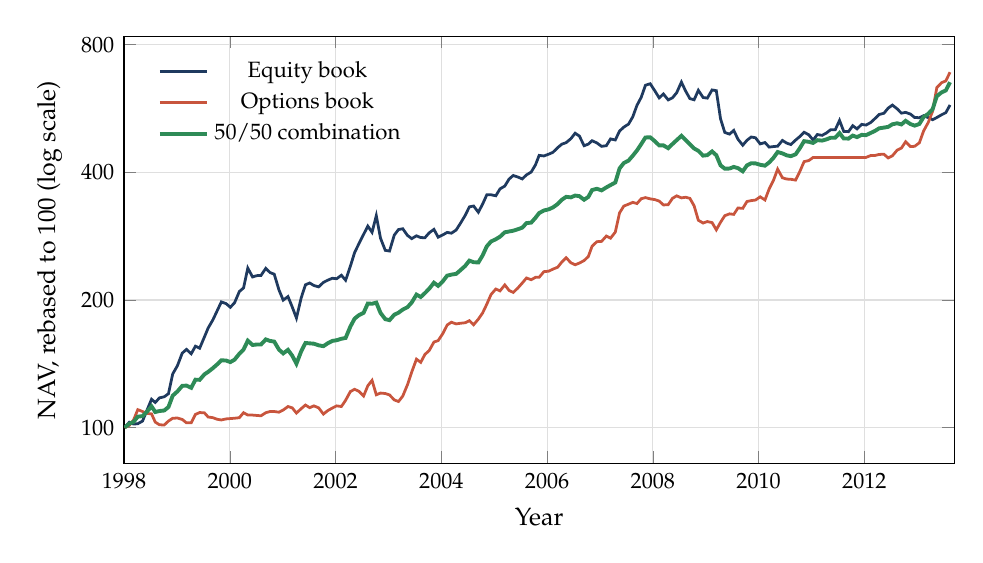
\begin{tikzpicture}
\begin{axis}[pead,height=7cm,ymode=log,xlabel={Year},ylabel={NAV, rebased to 100 (log scale)},
  xmin=1998,xmax=2013.7,xticklabel style={/pgf/number format/1000 sep={}},legend pos=north west,ytick={100,200,400,800},yticklabels={100,200,400,800}]
\addplot[color=cEq,line width=1pt] coordinates {(1998.01,100.1) (1998.10,103.0) (1998.18,102.0) (1998.26,102.2) (1998.35,103.7) (1998.43,109.7) (1998.52,116.7) (1998.59,114.7) (1998.67,117.6) (1998.76,118.3) (1998.84,120.3) (1998.92,133.9) (1999.01,140.1) (1999.10,149.9) (1999.18,153.0) (1999.27,149.4) (1999.35,155.7) (1999.43,154.0) (1999.52,163.7) (1999.59,171.8) (1999.68,179.6) (1999.76,188.6) (1999.84,198.0) (1999.93,196.1) (2000.01,192.3) (2000.09,197.1) (2000.18,209.4) (2000.26,213.6) (2000.34,237.8) (2000.43,226.7) (2000.51,228.3) (2000.59,228.6) (2000.68,237.5) (2000.76,232.2) (2000.84,230.1) (2000.93,211.2) (2001.01,199.9) (2001.10,203.8) (2001.18,192.7) (2001.26,181.4) (2001.35,202.4) (2001.43,217.2) (2001.51,219.4) (2001.59,216.4) (2001.68,214.8) (2001.77,220.1) (2001.85,222.7) (2001.94,225.1) (2002.02,224.5) (2002.11,228.8) (2002.19,222.7) (2002.28,240.3) (2002.36,258.8) (2002.44,271.3) (2002.53,285.6) (2002.61,298.7) (2002.69,288.9) (2002.77,316.1) (2002.85,279.7) (2002.94,261.9) (2003.02,260.9) (2003.11,284.5) (2003.19,293.2) (2003.27,294.5) (2003.36,284.0) (2003.44,279.1) (2003.53,283.4) (2003.61,280.7) (2003.69,280.5) (2003.77,288.0) (2003.86,293.5) (2003.94,281.3) (2004.03,284.9) (2004.11,288.7) (2004.19,287.5) (2004.28,292.5) (2004.36,303.1) (2004.45,316.5) (2004.53,331.6) (2004.61,333.2) (2004.70,322.1) (2004.78,336.5) (2004.86,354.1) (2004.94,354.1) (2005.03,352.2) (2005.11,365.7) (2005.20,371.3) (2005.28,385.5) (2005.36,393.3) (2005.45,389.8) (2005.53,386.0) (2005.61,394.5) (2005.70,400.7) (2005.78,416.5) (2005.85,438.5) (2005.94,437.2) (2006.03,441.4) (2006.11,445.8) (2006.20,457.3) (2006.28,466.2) (2006.36,469.9) (2006.45,480.2) (2006.53,494.6) (2006.61,487.2) (2006.70,462.1) (2006.78,466.2) (2006.85,474.9) (2006.94,469.3) (2007.03,460.6) (2007.12,462.2) (2007.20,479.5) (2007.29,476.8) (2007.37,500.4) (2007.45,511.1) (2007.54,519.7) (2007.62,540.5) (2007.70,575.6) (2007.78,601.1) (2007.86,641.7) (2007.95,647.0) (2008.04,621.8) (2008.12,599.2) (2008.20,612.0) (2008.29,592.7) (2008.37,599.2) (2008.45,616.1) (2008.54,652.7) (2008.62,621.8) (2008.70,596.9) (2008.78,593.0) (2008.86,624.4) (2008.95,600.4) (2009.03,598.4) (2009.12,625.6) (2009.20,623.1) (2009.28,534.8) (2009.36,496.7) (2009.45,492.2) (2009.53,502.2) (2009.61,478.6) (2009.70,463.4) (2009.78,476.0) (2009.86,484.6) (2009.94,482.6) (2010.03,466.7) (2010.12,470.2) (2010.20,458.7) (2010.28,460.0) (2010.36,461.0) (2010.45,475.6) (2010.53,468.8) (2010.61,465.2) (2010.70,476.5) (2010.78,485.9) (2010.86,497.2) (2010.95,490.3) (2011.03,476.6) (2011.11,491.1) (2011.20,488.9) (2011.28,495.0) (2011.36,503.9) (2011.45,504.3) (2011.53,530.1) (2011.61,499.5) (2011.70,498.8) (2011.78,515.2) (2011.86,506.4) (2011.95,518.9) (2012.03,516.9) (2012.12,524.2) (2012.20,535.5) (2012.28,547.5) (2012.37,551.2) (2012.45,566.8) (2012.53,576.2) (2012.62,564.6) (2012.70,551.5) (2012.78,553.8) (2012.87,548.8) (2012.95,538.7) (2013.04,538.0) (2013.12,544.0) (2013.21,538.1) (2013.29,532.2) (2013.37,538.6) (2013.46,546.7) (2013.54,553.0) (2013.62,576.5)};
\addplot[color=cOp,line width=1pt] coordinates {(1998.01,100.0) (1998.10,101.3) (1998.18,104.3) (1998.26,110.3) (1998.35,109.2) (1998.43,108.1) (1998.52,107.8) (1998.59,103.1) (1998.67,101.6) (1998.76,101.5) (1998.84,103.7) (1998.92,105.3) (1999.01,105.4) (1999.10,104.6) (1999.18,102.7) (1999.27,102.7) (1999.35,107.5) (1999.43,108.6) (1999.52,108.4) (1999.59,106.0) (1999.68,105.6) (1999.76,104.7) (1999.84,104.3) (1999.93,104.9) (2000.01,105.1) (2000.09,105.3) (2000.18,105.6) (2000.26,108.5) (2000.34,107.1) (2000.43,107.1) (2000.51,106.9) (2000.59,106.7) (2000.68,108.5) (2000.76,109.2) (2000.84,109.2) (2000.93,108.8) (2001.01,110.1) (2001.10,112.2) (2001.18,111.4) (2001.26,108.3) (2001.35,110.9) (2001.43,113.1) (2001.51,111.5) (2001.59,112.6) (2001.68,111.4) (2001.77,107.7) (2001.85,109.7) (2001.94,111.3) (2002.02,112.6) (2002.11,112.2) (2002.19,116.1) (2002.28,121.7) (2002.36,123.2) (2002.44,121.9) (2002.53,118.8) (2002.61,125.6) (2002.69,129.3) (2002.77,119.6) (2002.85,120.7) (2002.94,120.4) (2003.02,119.5) (2003.11,116.3) (2003.19,115.3) (2003.27,118.7) (2003.36,126.3) (2003.44,135.3) (2003.53,145.1) (2003.61,142.6) (2003.69,148.9) (2003.77,152.0) (2003.86,159.2) (2003.94,160.5) (2004.03,166.8) (2004.11,174.6) (2004.19,177.3) (2004.28,175.7) (2004.36,176.3) (2004.45,176.8) (2004.53,178.8) (2004.61,174.9) (2004.70,180.3) (2004.78,186.4) (2004.86,195.6) (2004.94,206.1) (2005.03,212.3) (2005.11,210.2) (2005.20,217.1) (2005.28,210.8) (2005.36,208.4) (2005.45,213.7) (2005.53,219.3) (2005.61,225.4) (2005.70,223.3) (2005.78,226.2) (2005.85,226.3) (2005.94,233.3) (2006.03,233.9) (2006.11,236.5) (2006.20,239.0) (2006.28,245.9) (2006.36,251.6) (2006.45,244.8) (2006.53,242.2) (2006.61,244.4) (2006.70,247.8) (2006.78,253.3) (2006.85,267.7) (2006.94,274.5) (2007.03,275.0) (2007.12,283.0) (2007.20,279.8) (2007.29,289.2) (2007.37,320.9) (2007.45,333.0) (2007.54,336.5) (2007.62,339.8) (2007.70,337.7) (2007.78,346.6) (2007.86,348.7) (2007.95,346.4) (2008.04,344.9) (2008.12,342.2) (2008.20,335.1) (2008.29,335.6) (2008.37,347.2) (2008.45,352.1) (2008.54,348.2) (2008.62,349.4) (2008.70,347.3) (2008.78,333.6) (2008.86,308.4) (2008.95,303.8) (2009.03,306.2) (2009.12,304.5) (2009.20,292.8) (2009.28,305.0) (2009.36,316.1) (2009.45,319.3) (2009.53,318.4) (2009.61,329.6) (2009.70,329.0) (2009.78,341.4) (2009.86,343.1) (2009.94,344.1) (2010.03,350.2) (2010.12,344.3) (2010.20,365.6) (2010.28,382.8) (2010.36,406.9) (2010.45,388.4) (2010.53,385.7) (2010.61,385.2) (2010.70,383.5) (2010.78,402.0) (2010.86,423.9) (2010.95,426.5) (2011.03,433.6) (2011.11,433.6) (2011.20,433.6) (2011.28,433.6) (2011.36,433.6) (2011.45,433.6) (2011.53,433.6) (2011.61,433.6) (2011.70,433.6) (2011.78,433.6) (2011.86,433.6) (2011.95,433.6) (2012.03,433.7) (2012.12,438.2) (2012.20,438.3) (2012.28,440.8) (2012.37,441.3) (2012.45,432.5) (2012.53,437.6) (2012.62,451.2) (2012.70,456.2) (2012.78,472.1) (2012.87,460.2) (2012.95,460.6) (2013.04,469.6) (2013.12,500.7) (2013.21,525.0) (2013.29,557.2) (2013.37,633.7) (2013.46,650.7) (2013.54,657.0) (2013.62,688.9)};
\addplot[color=cBl,line width=1.4pt] coordinates {(1998.01,100.1) (1998.10,102.2) (1998.18,103.2) (1998.26,106.2) (1998.35,106.5) (1998.43,109.0) (1998.52,112.3) (1998.59,108.9) (1998.67,109.5) (1998.76,109.8) (1998.84,111.9) (1998.92,119.0) (1999.01,121.8) (1999.10,125.5) (1999.18,125.7) (1999.27,124.2) (1999.35,129.8) (1999.43,129.7) (1999.52,133.6) (1999.59,135.4) (1999.68,138.2) (1999.76,141.0) (1999.84,144.2) (1999.93,144.0) (2000.01,142.8) (2000.09,144.7) (2000.18,149.4) (2000.26,152.9) (2000.34,160.4) (2000.43,156.7) (2000.51,157.1) (2000.59,157.1) (2000.68,161.5) (2000.76,160.2) (2000.84,159.6) (2000.93,152.8) (2001.01,149.7) (2001.10,152.6) (2001.18,147.9) (2001.26,141.6) (2001.35,151.4) (2001.43,158.4) (2001.51,158.1) (2001.59,157.8) (2001.68,156.4) (2001.77,155.7) (2001.85,158.1) (2001.94,160.2) (2002.02,160.8) (2002.11,162.1) (2002.19,162.8) (2002.28,173.2) (2002.36,180.8) (2002.44,184.2) (2002.53,186.6) (2002.61,196.3) (2002.69,196.0) (2002.77,197.3) (2002.85,186.5) (2002.94,180.3) (2003.02,179.3) (2003.11,184.7) (2003.19,186.7) (2003.27,189.9) (2003.36,192.4) (2003.44,197.4) (2003.53,206.0) (2003.61,203.3) (2003.69,207.7) (2003.77,212.6) (2003.86,219.7) (2003.94,216.0) (2004.03,221.6) (2004.11,228.3) (2004.19,229.6) (2004.28,230.5) (2004.36,235.1) (2004.45,240.6) (2004.53,247.7) (2004.61,245.6) (2004.70,245.2) (2004.78,254.7) (2004.86,267.7) (2004.94,274.8) (2005.03,278.2) (2005.11,282.1) (2005.20,288.9) (2005.28,290.1) (2005.36,291.4) (2005.45,293.8) (2005.53,296.2) (2005.61,303.6) (2005.70,304.5) (2005.78,312.5) (2005.85,320.7) (2005.94,325.2) (2006.03,327.2) (2006.11,330.6) (2006.20,336.7) (2006.28,344.8) (2006.36,350.2) (2006.45,349.2) (2006.53,352.6) (2006.61,351.5) (2006.70,344.7) (2006.78,350.1) (2006.85,363.3) (2006.94,365.8) (2007.03,362.7) (2007.12,368.6) (2007.20,373.3) (2007.29,378.5) (2007.37,408.5) (2007.45,420.6) (2007.54,426.3) (2007.62,437.7) (2007.70,450.4) (2007.78,466.3) (2007.86,483.3) (2007.95,483.8) (2008.04,473.3) (2008.12,462.9) (2008.20,463.0) (2008.29,456.0) (2008.37,466.3) (2008.45,476.3) (2008.54,487.6) (2008.62,476.8) (2008.70,465.9) (2008.78,455.3) (2008.86,449.5) (2008.95,438.0) (2009.03,439.1) (2009.12,448.0) (2009.20,438.9) (2009.28,415.5) (2009.36,408.0) (2009.45,408.3) (2009.53,411.9) (2009.61,409.2) (2009.70,402.3) (2009.78,415.4) (2009.86,420.2) (2009.94,419.9) (2010.03,416.7) (2010.12,414.7) (2010.20,422.1) (2010.28,432.6) (2010.36,446.6) (2010.45,443.3) (2010.53,438.7) (2010.61,436.7) (2010.70,441.1) (2010.78,456.1) (2010.86,473.7) (2010.95,472.0) (2011.03,469.2) (2011.11,476.3) (2011.20,475.2) (2011.28,478.2) (2011.36,482.5) (2011.45,482.8) (2011.53,495.0) (2011.61,480.6) (2011.70,480.4) (2011.78,488.3) (2011.86,484.2) (2011.95,490.2) (2012.03,489.4) (2012.12,495.3) (2012.20,500.8) (2012.28,507.9) (2012.37,509.9) (2012.45,511.9) (2012.53,519.2) (2012.62,522.0) (2012.70,518.8) (2012.78,528.9) (2012.87,519.9) (2012.95,515.4) (2013.04,520.0) (2013.12,540.0) (2013.21,550.0) (2013.29,563.5) (2013.37,604.6) (2013.46,617.4) (2013.54,623.9) (2013.62,652.5)};
\legend{Equity book,Options book,50/50 combination}
\end{axis}
\end{tikzpicture}
\caption{Growth of \$100 invested in each book and in their 50/50 daily-rebalanced
combination, January 1998 to August 2013. The options book is held in cash until its
return law has enough history, so the common window starts in 1998.}\label{fig:nav}
\end{figure}

\begin{table}[t]\centering\small
\caption{Risk profile of the two books. Rows marked $\ddagger$ are computed over each book's
active period from its daily return series.}\label{tab:risk}
\begin{tabular}{lrr}
\toprule
 & Equity book & Options book\\
\midrule
Annualized return & 12.15\% & 12.26\%\\
Annualized volatility & 12.20\% & 3.33\%\\
Sharpe ratio & 1.00 & 3.49\\
Maximum drawdown (trough date) & $-36.5\%$ (2010-05) & $-17.4\%$ (2009-03)\\
Final NAV from \$10M & \$93.3M & \$68.8M\\
\midrule
Sortino ratio$^\ddagger$ & 1.39 & 5.88\\
Skewness / kurtosis of daily returns$^\ddagger$ & $-0.22$ / 10.1 & $+0.99$ / 11.0\\
Daily 99\% VaR / CVaR$^\ddagger$ & $-2.13\%$ / $-3.05\%$ & $-0.48\%$ / $-0.70\%$\\
Market beta / correlation$^\ddagger$ & $-0.015$ / $-0.02$ & $0.034$ / $0.20$\\
CAPM alpha, annualized ($t$-stat)$^\ddagger$ & 13.0\% (4.47) & 12.9\% (14.26)\\
Calmar ratio$^\ddagger$ & 0.35 & 0.81\\
\bottomrule
\end{tabular}
\end{table}

The two books reach similar returns through different distributions (Table~\ref{tab:risk}).
The equity book is linear and hedged: negative skew, fatter left tail, no market exposure.
The options book is convex and budgeted: positive skew, daily tail losses about four times
smaller, and a loss bound set by construction (Proposition~\ref{prop:fractional}c). For both
books the CAPM alpha is essentially the entire return, so neither return is compensation for
market risk.

\subsection{Why the combination is better than either book}

Let the books have returns with annualized volatilities $\sigma_e,\sigma_o$, correlation
$\rho$, and a combination weight $w$ on equity. The combination's volatility is
\begin{equation}
  \sigma_p^2=w^2\sigma_e^2+(1-w)^2\sigma_o^2+2w(1-w)\rho\,\sigma_e\sigma_o.
  \label{eq:blendvar}
\end{equation}
Over the common window, $\sigma_e=12.68\%$, $\sigma_o=3.44\%$, and the daily correlation is
$\rho=-0.055$ (monthly: $-0.12$ over 175 months). Equation~\eqref{eq:blendvar} at $w=\tfrac12$
gives $\sigma_p=6.48\%$, matching the realized value. The cross term is negative, so
combining the books reduces risk below the root-mean-square of the individual risks, and
the combination's return is the average of the two.

The correlation is low for an economic reason. Both books earn from the same events, but the
equity book's short leg loses in a rally led by low-quality, heavily shorted stocks, the same
regime that produces momentum crashes \citep{DanielMoskowitz2016}, and it has no cap on that
loss. A purchased put loses at most its premium, and calls on positive-surprise names
participate in the rally. In 2009 the equity book lost $23.2\%$ while the options book gained
$14.3\%$ (Table~\ref{tab:calendar}, Figure~\ref{fig:cal}).

\begin{table}[t]\centering\small
\caption{Calendar-year returns (\%). The options book starts in 1998 once its return law has
history; its 2013 figure covers January to August.}\label{tab:calendar}
\begin{tabular}{lrrr@{\hspace{2em}}lrrr}
\toprule
Year & Equity & Options & Market & Year & Equity & Options & Market\\
\midrule
1996 & 33.1 & -- & 21.3 & 2005 & 23.0 & 9.7 & 7.3\\
1997 & 26.1 & -- & 30.4 & 2006 & 5.0 & 17.8 & 16.2\\
1998 & 37.1 & 5.4 & 22.3 & 2007 & 37.3 & 25.9 & 7.4\\
1999 & 35.9 & $-0.5$ & 25.7 & 2008 & $-1.6$ & $-12.0$ & $-38.2$\\
2000 & 12.6 & 4.9 & $-11.3$ & 2009 & $-23.2$ & 14.3 & 31.2\\
2001 & 2.8 & 2.2 & $-11.0$ & 2010 & $-0.1$ & 24.5 & 17.7\\
2002 & 18.7 & 6.4 & $-20.9$ & 2011 & 9.6 & -- & $-1.1$\\
2003 & 6.1 & 38.5 & 33.2 & 2012 & 2.2 & 7.1 & 15.8\\
2004 & 25.9 & 28.5 & 13.0 & 2013 & 7.4 & 48.3 & 30.5\\
\bottomrule
\end{tabular}
\end{table}

\begin{figure}[t]\centering
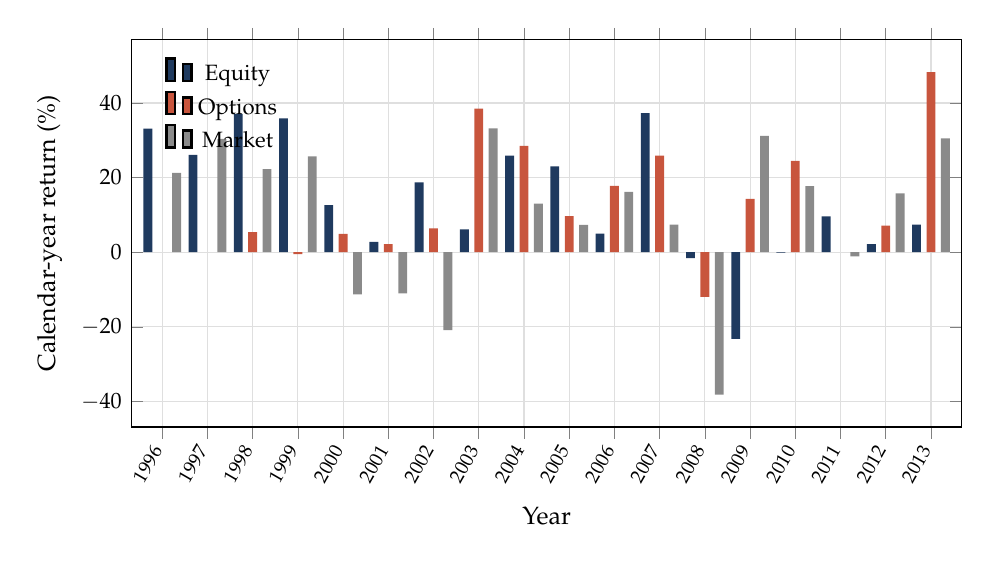
\begin{tikzpicture}
\begin{axis}[pead,ybar,bar width=3.2pt,height=6.5cm,xlabel={Year},ylabel={Calendar-year return (\%)},
  symbolic x coords={1996,1997,1998,1999,2000,2001,2002,2003,2004,2005,2006,2007,2008,2009,2010,2011,2012,2013},
  xtick=data,x tick label style={rotate=60,anchor=east,font=\scriptsize},legend pos=north west,
  enlarge x limits=0.04,ymajorgrids]
\addplot[fill=cEq,draw=none] coordinates {(1996,33.1)(1997,26.1)(1998,37.1)(1999,35.9)(2000,12.6)(2001,2.8)(2002,18.7)(2003,6.1)(2004,25.9)(2005,23.0)(2006,5.0)(2007,37.3)(2008,-1.6)(2009,-23.2)(2010,-0.1)(2011,9.6)(2012,2.2)(2013,7.4)};
\addplot[fill=cOp,draw=none] coordinates {(1998,5.4)(1999,-0.5)(2000,4.9)(2001,2.2)(2002,6.4)(2003,38.5)(2004,28.5)(2005,9.7)(2006,17.8)(2007,25.9)(2008,-12.0)(2009,14.3)(2010,24.5)(2012,7.1)(2013,48.3)};
\addplot[fill=cMk,draw=none] coordinates {(1996,21.3)(1997,30.4)(1998,22.3)(1999,25.7)(2000,-11.3)(2001,-11.0)(2002,-20.9)(2003,33.2)(2004,13.0)(2005,7.3)(2006,16.2)(2007,7.4)(2008,-38.2)(2009,31.2)(2010,17.7)(2011,-1.1)(2012,15.8)(2013,30.5)};
\legend{Equity,Options,Market}
\end{axis}
\end{tikzpicture}
\caption{Calendar-year returns of both books against the CRSP value-weighted market.}\label{fig:cal}
\end{figure}

\subsection{Combined performance}

\begin{table}[t]\centering\small
\caption{Static combinations of the two books, rebalanced daily, January 1998 to August 2013.}\label{tab:blend}
\begin{tabular}{rrrrr}
\toprule
Equity weight & CAGR & Vol & Sharpe & Max DD\\
\midrule
100\% & 11.82\% & 12.68\% & 0.94 & $-36.5\%$\\
75\% & 12.33\% & 9.50\% & 1.27 & $-25.6\%$\\
50\% & 12.73\% & 6.48\% & 1.88 & $-18.5\%$\\
25\% & 12.99\% & 3.98\% & 3.09 & $-15.0\%$\\
0\% & 13.13\% & 3.44\% & 3.61 & $-17.4\%$\\
\bottomrule
\end{tabular}
\end{table}

Table~\ref{tab:blend} shows the effect. At 50/50 the combination keeps the return of either
book ($12.7\%$ a year), doubles the equity book's Sharpe ratio ($0.94\to1.88$ over this window),
and halves its maximum drawdown ($-36.5\%\to-18.5\%$). The risk reduction comes from the
low correlation, not from giving up return. A fund can therefore choose its risk level by
moving along the table, or by scaling the whole combination, without changing the source of
return. The two books also diversify model risk: they use different instruments and rest on
different return distributions, so a balanced allocation is a natural default.

%=====================================================================================
\section{Conclusion}
%=====================================================================================

Post-earnings-announcement drift is a gradual incorporation of earnings news by
heterogeneously attentive investors. The model predicts a spread that rises concavely with
the horizon, is largest where arbitrage is costly, and is amplified by leverage in options. The
data confirm each prediction: the spread is significant under earnings-season clustering,
grows when size and value are controlled for, is graded by firm size, and appears in option
premia at the magnitude implied by elasticity.

Two strategies harvest this drift. The equity book earns it linearly: rank-proportional
positions, neutral to industry and size, held for the decay time of the drift, and scaled
to its capacity optimum. It earns about 12\% a year without market exposure. The options
book earns it convexly: it chooses for each event the contract that maximizes expected
log growth, and it sizes the portfolio as a deeply fractional Kelly book under a premium
budget. It also earns about 12\% a year, with a Sharpe ratio driven by breadth and losses
bounded by construction. The two books are nearly uncorrelated, and combined they
double the equity book's Sharpe ratio and halve its drawdown at no cost in return.

\vspace{1em}
\noindent\fbox{\parbox{\dimexpr\linewidth-2\fboxsep-2\fboxrule}{\footnotesize
\textbf{Disclosure.} All performance figures are hypothetical, are based on historical
backtests (1996--2013) net of modeled trading costs, and do not reflect actual trading.
Realized results may differ materially. Nothing here is an offer, a solicitation, or
investment advice.}}

%=====================================================================================
\appendix
\section{Proofs}\label{app:proofs}
%=====================================================================================

\paragraph{Concavity of the incorporation profile.}
A Gamma$(k,\theta)$ mixture of exponential rates has Laplace transform
$\E[e^{-\kappa d}]=(1+d/\theta)^{-k}$, which gives \eqref{eq:phi}. Then
$\phi'(d)=(1-\phi(0))\,(k/\theta)\,(1+d/\theta)^{-k-1}>0$ and $\phi''(d)<0$, so $\phi$ is
increasing and strictly concave with $\phi(d)\to1$. Since $\Delta(h)\propto\phi(h)-\phi(0)$,
the spread is increasing, concave and bounded. The unincorporated fraction decays as a
power, $(1+d/\theta)^{-k}$, not exponentially, so the profile has no single time scale and
keeps rising long after a single-speed model would have flattened.

\paragraph{Uniqueness of the holding period.}
Write $\mathcal Y(H)=(a(H)-k)/H$ with $a$ increasing and concave, $a(0)=0$, and
$a(\infty)>k$. Then $\mathcal Y'(H)=N(H)/H^2$ with $N(H)=a'(H)H-a(H)+k$, and $N(H)=0$ if and
only if $a'(H)=\mathcal Y(H)$. Now $N'(H)=a''(H)H<0$, $N(0)=k>0$, and
$N(H)\to k-a(\infty)<0$ as $H\to\infty$ (because $a'(H)H\to0$ for a concave bounded $a$).
So $N$ has exactly one zero $H^\ast$, and $\mathcal Y$ increases before it and decreases after,
which makes $H^\ast$ the unique maximizer. $\square$

\paragraph{Proof of Proposition~\ref{prop:neutral}.}
Fix $q$ and side $\sigma$. For an occupied group $g$,
$\sum_{i\in g}|\tilde w_i|=\sum_{i\in g}|t_i|\big/\big(\sum_{j\in g}|t_j|\cdot N_{q\sigma}\big)=1/N_{q\sigma}$,
which proves (b). Summing over the $N_{q\sigma}$ groups on a side gives
$\sum_{i\in q\sigma}|\tilde w_i|=1$ for both sides. Every weight on a side has the same sign,
so the long gross equals the short gross, and the global rescaling in \eqref{eq:weights}
multiplies all weights by one positive constant, which proves (a). For (c), industry $k$'s
long gross is the sum over its occupied long groups, $n^+_k/N_{q+}$, and likewise on the short
side. Net exposure is the difference, and it vanishes when $n^{+}_{k}/N_{q+}=n^{-}_{k}/N_{q-}$,
in particular when both sides occupy the same set of groups. The size argument is symmetric. $\square$

\paragraph{Proof of Proposition~\ref{prop:capacity}.}
Let the notional of position $i$ be $n_i=\min(|w_i|\,bV,\,\ell_i)$, where $\ell_i$ is its
liquidity limit. Position $i$ stops absorbing marginal capital at $b_i=\ell_i/(|w_i|V)$,
which increases in liquidity. Write $\mathcal U(b)=\{i:b<b_i\}$ for the uncapped set, which
shrinks as $b$ grows. The marginal alpha per marginal gross dollar is the $|w|$-weighted
average of $\alpha_i$ over $\mathcal U(b)$. Raising $b$ removes the members with the smallest
$b_i$, which are the least liquid names and, by assumption, those with the largest $\alpha_i$.
The weighted average therefore cannot increase, so expected arithmetic P\&L, the integral of
this non-increasing marginal alpha, is concave in $b$. Volatility is non-decreasing in
gross exposure, so $\mu(b)-\tfrac12\sigma^2(b)$ is concave with $\mu(0)=\sigma(0)=0$ and
positive slope at zero when the uncapped book has positive alpha. As $b\to\infty$ the alpha
saturates while the variance term does not, so the function eventually decreases and the
maximum is interior. $\square$

\paragraph{Proof of Proposition~\ref{prop:wellposed}.}
$R_{k,s}\ge-1$ and $f\le0.95$ give $1+fR_{k,s}\ge0.05$. The second derivative is
$G''_k(f)=-\sum_sp_sR_{k,s}^2/(1+fR_{k,s})^2<0$ unless every $R_{k,s}=0$. Direct evaluation
gives $G_k(0)=0$ and $G_k'(0)=\sum_sp_sR_{k,s}$. Since $G_k$ is concave, its maximizer on
$[0,1)$ is positive if and only if $G_k'(0)>0$. $\square$

\paragraph{Proof of Proposition~\ref{prop:sharpe}.}
Substitute $\log(1+y)=y-\tfrac12y^2+O(y^3)$ and take expectations, which gives
$G_k(f)=f\mu_k-\tfrac12f^2m_k+O(f^3\E|R_k|^3)$. Maximizing the quadratic gives
$f^\ast=\mu_k/m_k$ and $g^\ast=\mu_k^2/(2m_k)$. Dividing numerator and denominator by
$\sigma_k^2$ gives $\tfrac12\mathrm{SR}_k^2/(1+\mathrm{SR}_k^2)$, which is increasing in
$\mathrm{SR}_k$ for $\mathrm{SR}_k>0$. $\square$

\paragraph{Proof of Proposition~\ref{prop:hurdle}.}
$G_k$ is concave with $G_k(0)=0$. If $G_k(f_{\min})\le0$, concavity gives
$G_k(f)\le(f/f_{\min})\,G_k(f_{\min})\le0$ for every $f\ge f_{\min}$, so no stake on the grid has
positive growth and the contract cannot be selected. Selectability therefore requires
$G_k(f_{\min})>0$. In the quadratic approximation this reads
$f_{\min}\mu_k-\tfrac12f_{\min}^2m_k>0$, which is \eqref{eq:hurdle}. $\square$

\paragraph{Proof of Proposition~\ref{prop:fractional}.}
(a) is immediate from \eqref{eq:alloc}. (b) Under independence and the quadratic
approximation, portfolio growth is $\sum_i(\pi_i\mu_i-\tfrac12\pi_i^2m_i)$. Setting
$\pi_i=\lambda\mu_i/m_i$ gives
\[
\sum_i\frac{\mu_i^2}{m_i}\Big(\lambda-\tfrac12\lambda^2\Big)=(2\lambda-\lambda^2)\sum_ig^\ast_i .
\]
The portfolio mean is $\lambda\sum_i\mu_i^2/m_i$ and its standard deviation is
$\lambda(\sum_i\mu_i^2\sigma_i^2/m_i^2)^{1/2}$, so $\lambda$ cancels in the ratio. With $N$
bets of comparable size, the numerator is $O(N)$ and the denominator $O(\sqrt N)$. (c) A long
option position costs its premium and has a non-negative payoff, so its loss is at most the
premium, and premium outstanding is at most $cV_q$ by construction of $B_q$. $\square$

%=====================================================================================
\begin{thebibliography}{99}\small
%=====================================================================================
\bibitem[Ball and Brown(1968)]{BallBrown1968}
Ball, R., and P.~Brown (1968). An empirical evaluation of accounting income numbers.
\textit{Journal of Accounting Research} 6(2), 159--178.

\bibitem[Bernard and Thomas(1989)]{BernardThomas1989}
Bernard, V.~L., and J.~K.~Thomas (1989). Post-earnings-announcement drift: delayed price
response or risk premium? \textit{Journal of Accounting Research} 27 (Supplement), 1--36.

\bibitem[Bernard and Thomas(1990)]{BernardThomas1990}
Bernard, V.~L., and J.~K.~Thomas (1990). Evidence that stock prices do not fully reflect
the implications of current earnings for future earnings. \textit{Journal of Accounting and
Economics} 13(4), 305--340.

\bibitem[Daniel et~al.(1997)]{DGTW1997}
Daniel, K., M.~Grinblatt, S.~Titman, and R.~Wermers (1997). Measuring mutual fund
performance with characteristic-based benchmarks. \textit{Journal of Finance} 52(3),
1035--1058.

\bibitem[Daniel and Moskowitz(2016)]{DanielMoskowitz2016}
Daniel, K., and T.~J.~Moskowitz (2016). Momentum crashes. \textit{Journal of Financial
Economics} 122(2), 221--247.

\bibitem[DellaVigna and Pollet(2009)]{DellaVignaPollet2009}
DellaVigna, S., and J.~M.~Pollet (2009). Investor inattention and Friday earnings
announcements. \textit{Journal of Finance} 64(2), 709--749.

\bibitem[Fama and MacBeth(1973)]{FamaMacBeth1973}
Fama, E.~F., and J.~D.~MacBeth (1973). Risk, return, and equilibrium: empirical tests.
\textit{Journal of Political Economy} 81(3), 607--636.

\bibitem[Grinold(1989)]{Grinold1989}
Grinold, R.~C. (1989). The fundamental law of active management. \textit{Journal of
Portfolio Management} 15(3), 30--37.

\bibitem[Hirshleifer et~al.(2009)]{HirshleiferLimTeoh2009}
Hirshleifer, D., S.~S.~Lim, and S.~H.~Teoh (2009). Driven to distraction: extraneous events
and underreaction to earnings news. \textit{Journal of Finance} 64(5), 2289--2325.

\bibitem[Hong and Stein(1999)]{HongStein1999}
Hong, H., and J.~C.~Stein (1999). A unified theory of underreaction, momentum trading, and
overreaction in asset markets. \textit{Journal of Finance} 54(6), 2143--2184.

\bibitem[Kelly(1956)]{Kelly1956}
Kelly, J.~L. (1956). A new interpretation of information rate. \textit{Bell System
Technical Journal} 35(4), 917--926.

\bibitem[MacLean et~al.(2011)]{MacLeanThorpZiemba2011}
MacLean, L.~C., E.~O.~Thorp, and W.~T.~Ziemba, eds. (2011). \textit{The Kelly Capital Growth
Investment Criterion: Theory and Practice}. World Scientific.

\bibitem[Mendenhall(2004)]{Mendenhall2004}
Mendenhall, R.~R. (2004). Arbitrage risk and post-earnings-announcement drift.
\textit{Journal of Business} 77(4), 875--894.

\bibitem[Shleifer and Vishny(1997)]{ShleiferVishny1997}
Shleifer, A., and R.~W.~Vishny (1997). The limits of arbitrage. \textit{Journal of
Finance} 52(1), 35--55.
\end{thebibliography}

\end{document}
